\subsection{Arquitectura del Servidor}

A continuación, se presenta la arquitectura del
sistema integrando todos los módulos y las herramientas previamente seleccionadas.
Como se puede observar en la \cref{fig:Log1}, el Módulo 1 se comunicaran por medio de Wifi utilizando
el protocolo MQTT hacia el broker alojado en la nube utilzando el servicio de EMQX,
el cual se encargará de recibir los datos del Módulo 1. 
El Módulo 3 alamacenara los datos por medio de una base de datos en la nube en MongoDB,
y el Módulo 2 alojado de forma local se encargara de almacenar los datos.Por ultimo,
el Módulo 4 igualemente aloado de forma local se encargará de mostrar la información al los productores 
y administradores por medio de una aplicación web.


\begin{figure}[htb]
    \centering
    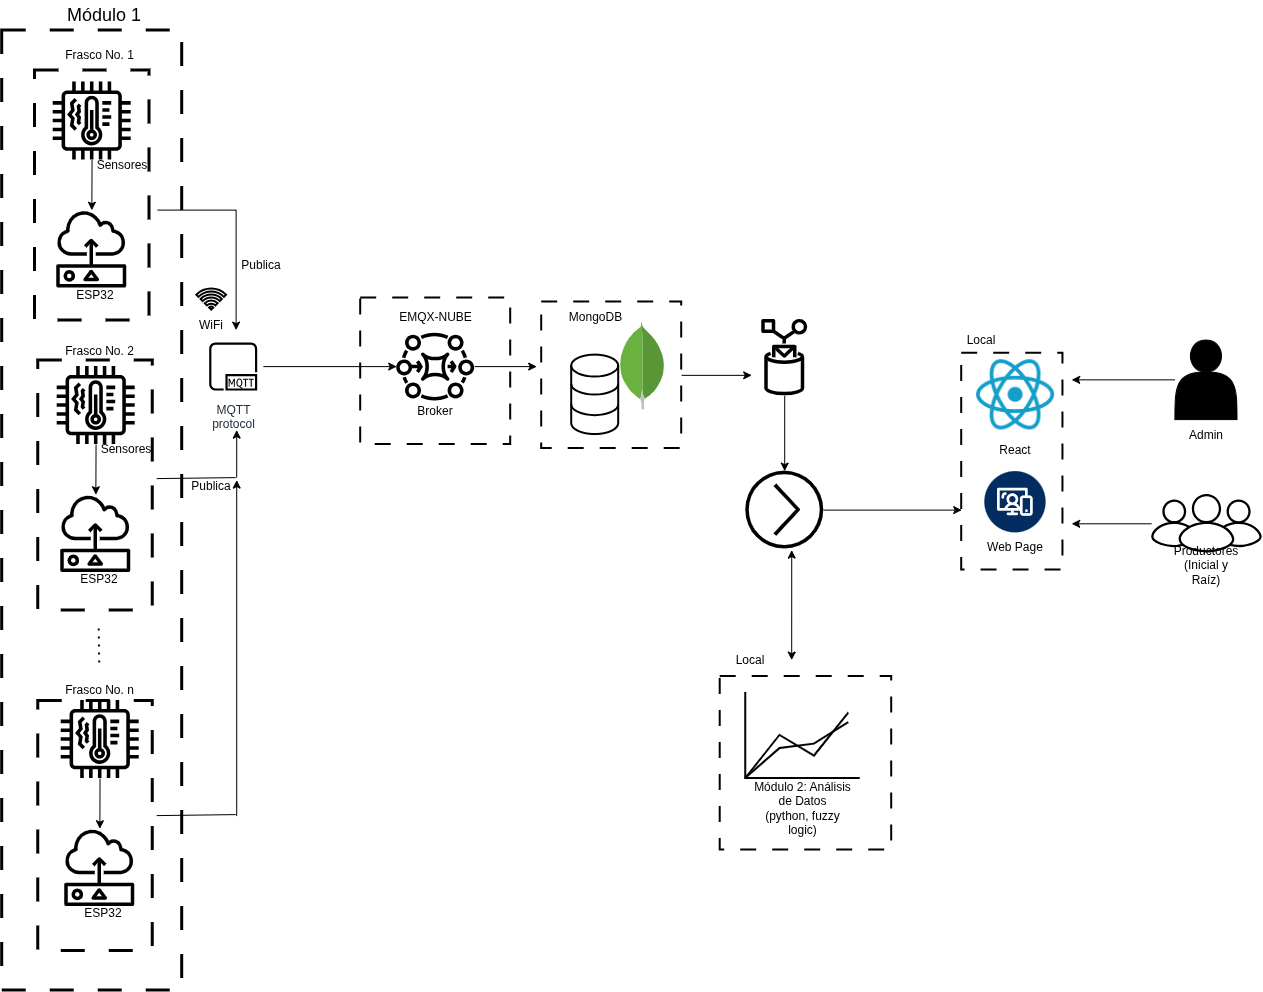
\includegraphics[width=1\textwidth]{./UML/Modulo4/arqui.drawio.png}
    \caption{Arquitectura del Servidor}
    \label{fig:Log1}
    \end{figure} 